% This is lnbip.tex the demonstration file of the LaTeX macro package for
% Lecture Notes in Business Information Processing from Springer-Verlag.
% It serves as a template for authors as well.
% version 1.0 for LaTeX2e
%
\documentclass[lnbip]{svmultln}
%
\usepackage{makeidx}  % allows for indexgeneration
\usepackage{graphicx}
\usepackage{booktabs}
\usepackage{multirow}
\usepackage{url}
\begin{document}
%
\mainmatter              % start of the contribution
%
\title{Toward Human-Centric Explainable AI: Integrating Large Language Models and Ontologies for Semantically Grounded Explanations}
%
\titlerunning{Human-Centric Ontology-Grounded Explainable AI}
%
\author{Mostaqim Murshed\inst{1} \and Madhushi Bandara\inst{1}}
%
\authorrunning{Murshed and Bandara}
%
\tocauthor{Mostaqim Murshed, Madhushi Bandara}
%
\institute{University of Technology Sydney, Sydney, Australia\\
\email{mostaqim.murshed@students.uts.edu.au}}

\maketitle

\begin{abstract}
This paper proposes the Human-Centric Ontology-Grounded Explanation (HOGE) framework, which integrates large language models (LLMs) with domain ontologies and knowledge graphs (KGs) to produce semantically grounded, audience-adaptive explanations for machine learning decisions. While Explainable AI (XAI) methods such as SHAP provide valuable technical transparency, their outputs remain difficult for non-technical stakeholders to interpret. LLMs can translate these outputs into natural language but risk hallucination and unfaithful reasoning. HOGE addresses this gap by positioning the ontology as a semantic contract that constrains what explanations can claim, and the LLM as a mediator that translates ontology-grounded evidence into human-consumable narratives. We prototype HOGE in a loan decisioning domain using XGBoost with monotonic constraints, SHAP feature attribution, a Neo4j knowledge graph, and GPT-4o as the narrative explainer. Empirical evaluation across 100~test-set applications demonstrates: average explanation faithfulness of 0.745, semantic fidelity of 0.740, evidence coverage of 0.921, hallucination rate of 26.0\%, perfect graph retrieval accuracy (Precision@K~=~1.0), 96\% SHAP--prediction alignment, and counterfactual single-feature flips for 93\% of tested applications. These results demonstrate HOGE's ability to deliver grounded, traceable, and human-readable explanations for high-stakes decisions.
\keywords{Explainable AI, Large Language Models, Ontology, Knowledge Graph, SHAP, Human-Centric AI, Semantic Grounding}
\end{abstract}
%
\section{Introduction}
Despite the rapid deployment of machine learning and AI systems in high-stakes domains, their effective adoption by everyday users remains fundamentally constrained by inadequate explanations. Existing XAI techniques largely prioritise technical transparency, producing artefacts such as feature attributions and saliency maps that may satisfy model developers but fail to support the needs of practitioners, auditors, regulators, and non-technical decision makers. This disconnect reflects a critical problem: interpretability is audience-dependent, yet most explanation methods are designed without regard for how humans actually reason about decisions---contrastively, selectively, and through domain-level concepts rather than raw statistics.

Recent advances in large language models appear to offer a solution by translating technical outputs into fluent, audience-adaptive narratives. However, LLM-generated explanations introduce serious risks, including hallucination, weak evidential grounding, and persuasive but unfaithful reasoning, particularly in regulated and domain-specific settings. Ontologies and knowledge graphs provide a complementary capability by encoding domain semantics, constraints, and relationships, but they are rarely leveraged as active explanation mechanisms and remain largely inaccessible to non-experts. As a result, current approaches force an unsatisfactory trade-off between technical fidelity and human usability.

This paper addresses this unresolved gap by arguing that human-centric explainability requires the principled integration of XAI, LLMs, and ontological grounding. Rather than treating these components in isolation, we contend that ontologies must actively constrain what explanations are allowed to claim, LLMs must operate as grounded mediators rather than free-form generators, and technical model evidence must be preserved end-to-end. Only through such integration can explanations become simultaneously faithful, auditable, and cognitively aligned with real human users.

This paper makes the following contributions:
\begin{enumerate}
    \item \textbf{A novel semantic-contract framing for explainable AI.}
    We introduce the Human-Centric Ontology-Grounded Explanation (HOGE) framework, which positions a domain ontology as a semantic contract that explicitly constrains what LLM-generated explanations are permitted to claim, governing explanation validity, limiting hallucination, and ensuring traceability to model evidence.

    \item \textbf{An end-to-end, human-centric explanation architecture.}
    We propose a complete explanation pipeline spanning predictive modelling, post-hoc feature attribution, ontology-driven knowledge graph construction, policy and risk rule binding, and constraint-aware LLM narrative generation, delivering explanations that are selective, contrastive, and audience-adaptive.

    \item \textbf{Ontology-grounded provenance and counterfactual explanations.}
    We model SHAP feature attributions, policy rules, risk factors, and counterfactual what-if scenarios as first-class nodes in a knowledge graph, enabling lossless provenance tracing from narrative claims back to model behaviour.

    \item \textbf{A rigorous evaluation framework beyond text similarity.}
    We operationalise a multi-level evaluation aligned with interpretability theory, including perturbation-based faithfulness testing, semantic fidelity, evidence coverage, hallucination characterisation under constraint, and graph retrieval precision.

    \item \textbf{Empirical validation in a regulated decision domain.}
    Through a loan decisioning prototype using monotonic XGBoost, SHAP, Neo4j, and GPT-4o, we demonstrate high explanation faithfulness (0.745), perfect graph retrieval accuracy (Precision@K = 1.0), strong semantic fidelity (0.740), and actionable counterfactual explanations with full auditability across 100~test-set applications.
\end{enumerate}

This paper is organised as follows. Section~2 reviews background and related work and identifies the research gap. Section~3 presents the methodology, Section~4 the HOGE architecture, Section~5 the prototype implementation, Section~6 the evaluation results, and Section~7 the discussion. Section~8 concludes the paper.


\section{Background and Related Work}

This section reviews the three research streams underpinning the proposed HOGE framework---Explainable AI, Large Language Models for explanation generation, and ontologies/knowledge graphs for semantic grounding---and synthesises their limitations to motivate the identified research gap.

\subsection{Explainable AI: From Technical Transparency to Human Understanding}

Explainable AI (XAI) has produced a wide range of techniques for increasing transparency of machine learning models. Post-hoc feature attribution methods such as SHAP~\cite{lundberg2017} and LIME~\cite{ribeiro2016} are now standard tools for local explanation, decomposing predictions into per-feature contributions. Recent work has extended these methods through hybrid architectures that combine feature attribution with domain knowledge or representation learning, enabling more meaningful interpretations in applied domains~\cite{dti2025,ncd2025}.

Despite these advances, a fundamental limitation persists: XAI outputs are typically numerical scores, saliency maps, or local approximations that require statistical literacy to interpret. Doshi-Velez and Kim~\cite{doshi2017} argued that interpretability is not an intrinsic property of a model, but a relationship between an explanation and its audience. Complementing this view, Miller~\cite{miller2019} demonstrated that human explanations are inherently contrastive, selective, and social---properties largely absent from standard XAI outputs. Surveys of hybrid neuro-symbolic approaches further suggest that incorporating prior knowledge can improve transparency and robustness compared to purely post-hoc explanations~\cite{priork2024}. Together, these insights highlight the need for explanation methods that support both technical fidelity and human understanding.

\subsection{Large Language Models as Explanation Mediators}

Large Language Models (LLMs) introduce a powerful capability for XAI by translating structured model outputs into fluent, audience-adaptive natural language explanations. Recent systems across cybersecurity, industrial diagnostics, and healthcare demonstrate that LLMs can summarise model behaviour, maintain conversational context, and generate structured rationales grounded in retrieved evidence~\cite{ddos2025,klage2026,cip2026,medsum2026,chimera2025,racds2026}.

However, LLM-generated explanations are prone to hallucination, particularly when claims are not tightly constrained by domain evidence. Even retrieval-augmented and GraphRAG-based approaches primarily improve information recall rather than governing what an explanation is allowed to assert. Empirical evidence shows that ontology-grounded explanation mechanisms can substantially reduce hallucination compared to unconstrained LLM outputs, underscoring the importance of structured semantic grounding~\cite{threat2025}. This limitation is critical in high-stakes domains, where explanations must be faithful, auditable, and normatively constrained rather than merely fluent.

\subsection{Ontologies and Knowledge Graphs for Semantic Grounding}

Ontologies and knowledge graphs provide a formal semantic layer for representing domain concepts, relationships, and constraints, enabling structured reasoning and traceability in AI systems. Confalonieri et al.~\cite{confalonieri2021} identified key roles of ontologies in XAI, including reference modelling, common-sense reasoning, and explanation scaffolding. Recent work demonstrates that ontology- and KG-grounded approaches improve transparency and reasoning coherence across domains such as complex system diagnostics, healthcare, and education~\cite{deibo2025,diag2025,gdm2026,synkg2025,learn2024,sop2025}.

Despite their strengths, most ontology-based approaches focus on retrieval or post-hoc reasoning support rather than actively constraining explanation generation. As a result, while knowledge graphs can inform explanations, they do not typically govern explanation validity when paired with probabilistic language models.

\subsection{Integrated Approaches Combining LLMs, KGs, and XAI}

A growing body of work integrates LLMs, knowledge graphs, and XAI to improve transparency and reasoning across application domains, including agriculture, healthcare, and e-government~\cite{seeds2025,soil2025,agri2025,medkgcot2025,depress2025,cognet2025,egov2025,hybridkg2025,compass2025}. These systems commonly use KGs to retrieve contextual information for LLM prompts or to structure intermediate reasoning steps, leading to improvements in factual accuracy and explanation coherence.

However, three limitations persist across existing integrated approaches. First, ontologies and KGs are typically used to augment LLM outputs rather than as normative constraints on what explanations may claim. Second, explanation pipelines are often incomplete, lacking end-to-end provenance from model outputs through narrative explanations. Third, evaluation practices rely heavily on text-similarity or task-accuracy metrics, which do not assess faithfulness to underlying model behaviour or domain constraints~\cite{gdm2026,medsum2026,medkgcot2025}. These limitations motivate the need for an explanation architecture in which domain knowledge explicitly governs explanation validity.


\section{Design Science Research Methodology}
We adopt the Design Science Research Methodology (DSRM) to guide the development of the proposed HOGE framework. DSRM is well suited for this research as we aim to create and evaluate an artifact designed to solve a practical problem and contribute knowledge to the field~\cite{peffers2007, hevner2004}.
Our findings in DSRM problem identification stage are discussed in Section 1 and 2 and led to formulate the following research questions that formalise our study objective:

\noindent\textbf{RQ1:} How can an ontology serve as a semantic contract that constrains LLM-generated explanations to only reference grounded evidence, and what is the resulting impact on hallucination rate?

\noindent\textbf{RQ2:} To what extent do ontology-grounded LLM explanations faithfully reflect the underlying ML model's reasoning, as measured through perturbation-based faithfulness testing?

\noindent\textbf{RQ3:} Can a knowledge graph-based evidence pipeline preserve complete explanation provenance and achieve lossless retrieval accuracy for feature attributions and policy rules?

Section 4 provides the design and development of HOGE, followed by its Demonstration and Evaluation in Sections 5 and 6.

\section{Proposed HOGE Architecture}
The HOGE system architecture consists of three major components: predictive modelling and technical explainer, semantic knowledge representation, and narrative explanation. Figure~\ref{fig:architecture} presents the high-level architecture of the HOGE framework, illustrating the data flow from the predictive model through the semantic knowledge layer to the narrative explainer.
\begin{figure}[htp]
    \centering
    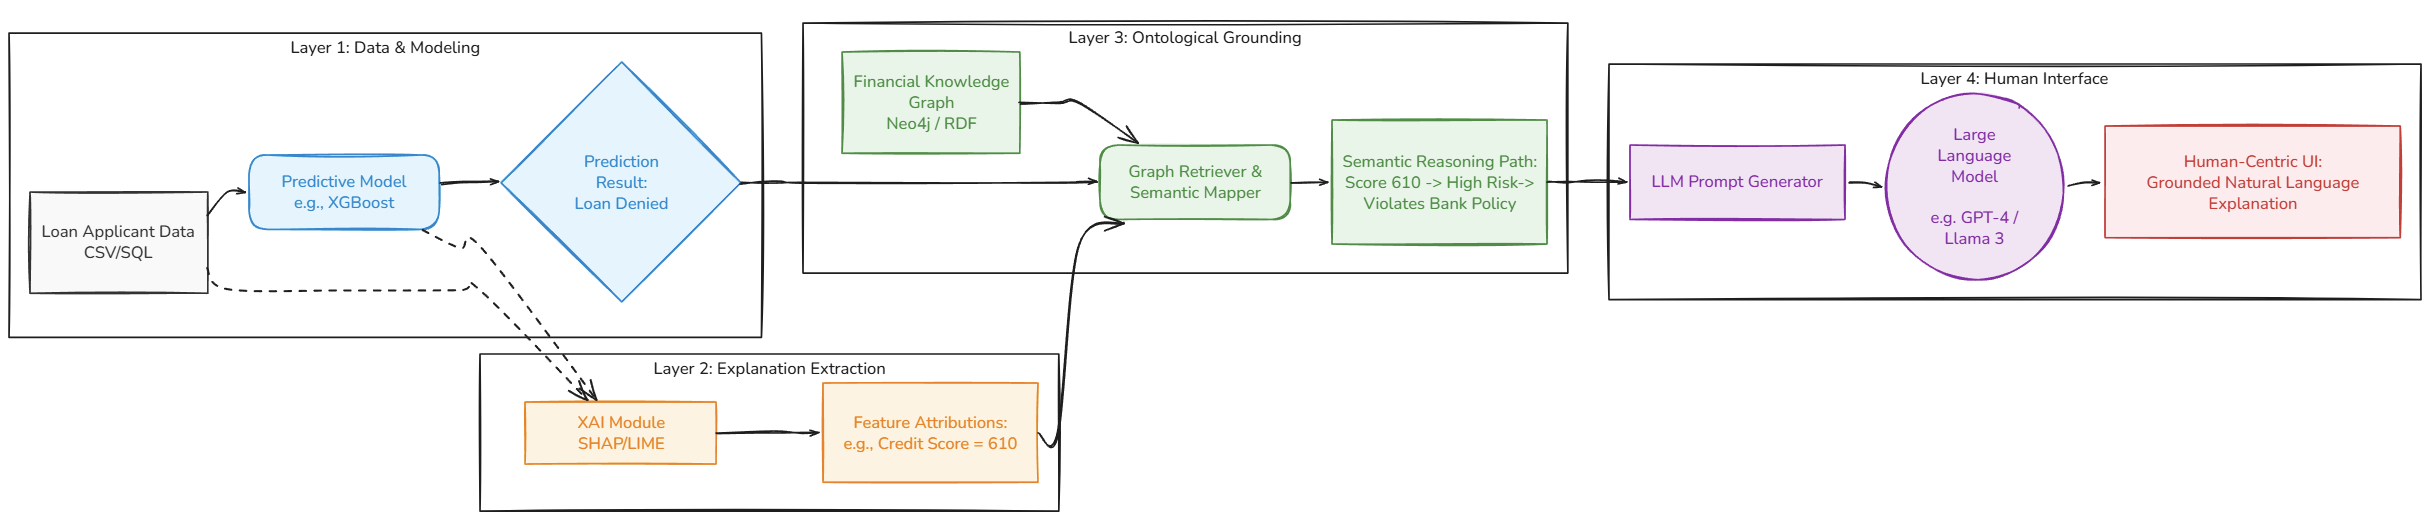
\includegraphics[width=\linewidth]{Architecture.png}
    \caption{HOGE system architecture: Component~A (Predictive Model and Technical Explainers), Component~B (Semantic Knowledge Representation), and Component~C (Narrative Explainer) interact to produce human-centric, ontology-grounded explanations.}
    \label{fig:architecture}
\end{figure}
\subsection{Component A: Predictive Model and Technical Explainers}

HOGE is designed to integrate into existing predictive models and model explainability methods. For example, explainability methods may include feature attribution (e.g., SHAP~\cite{lundberg2017}), local surrogate models (e.g., LIME~\cite{ribeiro2016}), counterfactual generation, and uncertainty estimation. HOGE does not replace technical XAI, but extends its capability.

\subsection{Component B: Semantic Knowledge Representation}
This component contains an ontology (schema) and a knowledge graph (KG) and support reasoning and traceability, consistent with the roles of ontologies in XAI described by Confalonieri and Guizzardi~\cite{confalonieri2021}.
The ontology defines domain concepts, relationships, constraints, and permissible explanation primitives.
Crucially, HOGE positions the ontology as a \emph{semantic contract} for explanation generation. The contract is operationally defined by three elements: (i)~the closed set of \texttt{Feature} nodes that enumerate every attribute the explanation may reference, (ii)~the \texttt{PolicyRule} and \texttt{RiskFactor} nodes that define permissible domain constraints, and (iii)~the grounding instruction embedded in the LLM prompt that prohibits claims about features or rules not present in the KG. Together, these elements constrain the LLM to produce explanations that are traceable to evidence rather than fabricated from parametric knowledge.

We ground the HOGE ontology on RVO model~\cite{rvo2019}, an ontology designed to catalogue machine learning process elements such as variables, analytics models and available data sources. RVO is extended in HOGE to capture unified representation necessary to support end-user friendly explanations. The main classes and relationships of HOGE ontology are represented in Figure~\ref{fig:HOGEontology}. Figure~\ref{fig:kg_schema} shows an instance of HOGE ontology for loan applications, implemented as a knowledge graph in Neo4j graph database.
\begin{figure}[htp]
    \centering
    \begin{minipage}[t]{0.48\linewidth}
        \centering
        \includegraphics[width=\linewidth]{HUGO-OntologyV1.pdf}
        \caption{The ontology for HOGE}
        \label{fig:HOGEontology}
    \end{minipage}\hfill
    \begin{minipage}[t]{0.48\linewidth}
        \centering
        
\includegraphics[width=\linewidth]{neo4j_kg_schema.png}
        \caption{Loan application represented through the HOGE KG}
        \label{fig:kg_schema}
    \end{minipage}
\end{figure}

The KG is populated via a six-stage ingestion pipeline that creates graph constraints, loads case-level nodes (Applicant, LoanApplication, demographic attributes), ingests model and explainer outputs (SHAP signed values, absolute importance, rank, direction), links feature values, attaches policy rules and risk factors with automatic violation detection, and persists counterfactual scenarios via \texttt{HAS\_COUNTERFACTUAL} and \texttt{PERTURBS\_FEATURE} relationships.

Each case has an explicit KG provenance path, e.g.\ \texttt{(LoanApplication) -[:HAS\_SHAP\_EXPLANATION]-> (ModelExplanation) -[:HAS\_CONTRIBUTION]-> (FeatureContribution) -[:FOR\_FEATURE]-> (Feature)}, enabling full traceability from any narrative claim back to its source. Counterfactual paths follow an analogous structure, ensuring contrastive what-if claims are also KG-grounded.

\subsection{Component C: Narrative Explainer}
The role of Narrative Explainer is to use LLM and generate explanations in natural language only operating within the concepts and claims provided through semantic knowledge representation layer. 
Its key function is to turn concept-evidence pairs into coherent narratives aligned with how humans understand explanations (contrastive, selective, and context-appropriate)~\cite{miller2019}.

The Narrative Explainer operates under strict grounding constraints: the prompt supplies ALL feature contributions ranked by importance, ALL policy rules from the domain ontology, and explicit instructions that the LLM may ONLY reference features and rules present in the evidence. The output is a structured JSON requiring summary, positive/negative drivers, policy violations, recommendation, counterfactual what-if, full narrative, and a self-reported feature list---enabling automated cross-checking. This explanation can be delivered through an interface supporting iterative questioning and progressive disclosure~\cite{miller2019}.

\section{Prototype Implementation}

\subsection{Case Study and Predictive Model}
We prototype HOGE in a loan decisioning domain using the publicly available Loan Eligible Dataset~\cite{kaggle_loan} (614~records). After pre-processing (removing incomplete records and engineering TotalIncome and Debt-to-Income ratio), 500~applications were retained. An XGBoost model with monotonic constraints---increasing income must not reduce approval probability, increasing DTI must not increase it, and improving credit history must never worsen risk---was trained on 22~transformed features including income, credit history, loan amount, tenure, DTI, and encoded categorical variables. The model achieved ROC-AUC of 0.839 on the held-out test set (20\% split, stratified) with overall accuracy of 80\%.


\subsection{Technical Explainer}
SHAP TreeExplainer was applied to decompose each prediction into per-feature contributions: signed SHAP values (positive $\rightarrow$ approval, negative $\rightarrow$ decline), absolute importance rankings (1--22), and direction labels. The long-format SHAP CSV (11,000 rows: one per application--feature pair) serves as the primary input for KG ingestion.

\subsection{Knowledge Graph Construction in Neo4j}
A Loan Explainability KG was constructed in Neo4j, comprising 500 LoanApplication nodes, 22 Feature types, 11,000 FeatureValue and FeatureContribution nodes, 500 ModelExplanation nodes, 2 PolicyRule nodes, 2 RiskFactor nodes, and CounterfactualScenario nodes for evaluated applications. Policy violations were automatically detected: applications with DTI~$>$~2.0 received \texttt{VIOLATES\_RULE} links to \texttt{RULE\_DTI\_001}, and those with \texttt{Credit\_History}~=~0 were linked to \texttt{RULE\_CREDIT\_001}. The KG supports multi-hop queries such as ``Which features most influenced Application~X?'' and ``What minimal change would flip the decision?''


\subsection{Narrative Explanation via Large Language Models}
We used GPT-4o with temperature=0.3 to implement the narrative explainer. It receives the full KG context for an application as a constraint-aware prompt. The prompt enumerates all 22~feature contributions, all known policy rules, and explicit grounding instructions prohibiting the LLM from inventing facts not present in the evidence.

The LLM output is a structured JSON containing summary, positive/negative drivers, policy violations, recommendation, a full narrative, and the list of referenced features. Each explanation is persisted with provenance metadata (model version, XAI method, KG loader version, HOGE version, UTC timestamp) and an evidence bundle mapping each claim to its KG path. For example, for application LP001006 (Approved, 91.1\%), the narrative highlights coapplicant income and credit history as positive drivers while noting lower applicant income and non-semiurban property as minor negative factors---each claim traceable to a specific KG node.

\section{Evaluation}

A central weakness in the current literature is that evaluation of explanation quality is often reduced to proxy metrics such as BLEU/ROUGE/BERTScore, which measure linguistic quality but not faithfulness to model behaviour~\cite{gdm2026,medsum2026,medkgcot2025}. We evaluate HOGE across three levels grounded in interpretability evaluation taxonomy~\cite{doshi2017}, as illustrated in Figure~\ref{fig:evalFramework}. Level~3 (real-world decision utility) is deferred to future work.

\begin{figure}[htp]
    \centering
    \includegraphics[width=0.8\linewidth]{HOGE_Evaluation_Framework.pdf}
    \caption{Evaluation framework utilised in HOGE}
    \label{fig:evalFramework}
\end{figure}

\begin{itemize}
    \item \textbf{Level~1 --- Semantic and Factual Grounding:}
    Quantitative evaluation of (A1) explanation faithfulness via perturbation tests,
    (A2) grounding precision and hallucination rate via claim-level verification, and
    (A3) graph retrieval accuracy via Precision@K.
    \item \textbf{Level~2 --- Human-Centric Evaluation:}
    Qualitative consistency checks covering SHAP--prediction alignment, end-to-end traceability of intermediate outcomes, and LLM grounding coverage against KG evidence.
\end{itemize}

All evaluations were conducted on 100~applications drawn from the held-out test split (20\% of 500 records) using stratified random sampling (seed=42). All results are reproducible via scripts provided in the project repository\footnote{\url{https://github.com/staq-6/Phd-Experiment1}}. Results are summarised in Table~\ref{tab:evalSummary}.

\subsection{A1. Explanation Faithfulness}

Faithfulness was assessed using perturbation-based testing, where the top SHAP feature for each application was perturbed and the resulting change in prediction and SHAP attribution was evaluated. An LLM-as-judge (GPT-4o, temperature~=~0) scored each case on a 0--1 scale based on directionality, magnitude plausibility, and driver consistency.

Across 98 tested applications (2 skipped due to zero-valued top features), the average faithfulness score was \textbf{0.745}, with 87/98 applications passing (score $\geq$~0.5, 88.8\%) and 48 achieving perfect faithfulness (49.0\%). Only 3 applications failed completely (score = 0.0, 3.1\%). Credit\_History perturbations produced the largest and most consistent probability shifts. The small number of failure cases revealed interactions between perturbation testing and feature scaling, discussed further in Section~\ref{sec:discussion}.

\subsection{A2. Grounding Precision and Hallucination Rate}

To assess grounding, generated explanations were decomposed into factual claims and verified against the full KG evidence bundle (features, SHAP values, policy rules, and predictions). Claims were classified as grounded, partially grounded, or hallucinated.

Across 100 applications, \textbf{Semantic Fidelity} averaged \textbf{0.740}, \textbf{Evidence Coverage} averaged \textbf{0.921}, and the \textbf{Hallucination Rate under Constraint} averaged \textbf{0.260}. Importantly, no explanations fabricated features or policy rules; hallucinations were limited to qualitative embellishments (e.g., ``the applicant's income is high''), indicating that the ontology effectively constrains factual claims.

\subsection{A3. Graph Retrieval Accuracy}

Graph retrieval accuracy validates the integrity of the KG ingestion pipeline. For each application, top-K features retrieved from Neo4j were compared against the SHAP CSV ground truth.

All 100 applications achieved \textbf{perfect scores}: Prediction Match~=~100\%, Precision@3~=~Precision@5~=~Precision@10~=~1.000, and Feature Recall~=~1.000. Policy rule retrieval was also correct for all applicable cases, confirming lossless provenance and reliable evidence retrieval.

\subsection{B. Human-Centric Evaluation}

Human-centric checks assess internal consistency, traceability, and alignment with model reasoning. SHAP--prediction alignment was verified for all 100 applications: 96 showed perfect directional consistency between the SHAP sum sign and the predicted class, and prediction accuracy against ground-truth labels was 99/100.

All eight pipeline stages---from raw features to LLM-generated explanations---were traceable via persisted JSON artefacts and a multi-sheet Excel workbook, enabling full auditability. LLM grounding analysis showed \textbf{98\% average coverage} of top-5 SHAP features, while overall coverage (including low-importance raw features) averaged \textbf{64\%}, reflecting selective explanation behaviour consistent with human explanation principles~\cite{miller2019}.

\subsection{C. Counterfactual Analysis}
\label{sec:counterfactual}

To support contrastive explanations (``Why A instead of B?''), HOGE incorporates a counterfactual explanation module that computes minimal actionable feature changes required to flip a prediction. Counterfactuals are persisted in the knowledge graph as \texttt{CounterfactualScenario} nodes linked to both the application and perturbed features, ensuring that contrastive what-if claims in the LLM narrative are grounded in KG-retrieved evidence.

Single-feature flips were identified for \textbf{93 of 100 applications (93\%)}, with \textit{Credit\_History} emerging as the most influential lever (72 cases), followed by CoapplicantIncome (12 cases) and LoanAmount (8 cases). The 7 non-flippable cases corresponded to highly robust predictions that could not be reversed through any single actionable feature change, providing useful confirmation signals. Persisting counterfactuals with explicit provenance enables contrastive explanations to be integrated into the LLM narrative with end-to-end traceability, operationalising Miller's contrastive property within HOGE.

\begin{table}[htp]
    \centering
    \caption{Summary of HOGE evaluation results across 100 test-set applications}
    \label{tab:evalSummary}
    \begin{tabular}{l l r}
        \toprule
        \textbf{Evaluation Axis} & \textbf{Metric} & \textbf{Result} \\
        \midrule
        \multirow{4}{*}{A1. Faithfulness}
            & Avg Faithfulness Score & 0.745 \\
            & Pass Rate ($\geq$ 0.5) & 87/98 (88.8\%) \\
            & Perfect Score (1.0) & 48/98 (49.0\%) \\
            & Failed (0.0) & 3/98 (3.1\%) \\
        \midrule
        \multirow{4}{*}{A2. Grounding}
            & Avg Semantic Fidelity (SF) & 0.740 \\
            & Avg Evidence Coverage (EC) & 0.921 \\
            & Avg Hallucination Rate (HRC) & 0.260 \\
            & Zero-Hallucination Apps & 0/100 \\
        \midrule
        \multirow{4}{*}{A3. Graph Retrieval}
            & Prediction Match Rate & 100/100 (100\%) \\
            & Avg Precision@3 & 1.000 \\
            & Avg Precision@5 & 1.000 \\
            & Avg Precision@10 & 1.000 \\
        \midrule
        \multirow{4}{*}{B. Human-Centric}
            & Prediction Accuracy & 99/100 (99\%) \\
            & SHAP--Prediction Alignment & 96/100 (96\%) \\
            & Avg SHAP Top-5 Coverage & 98\% \\
            & Avg Overall Coverage & 64\% \\
        \midrule
        \multirow{3}{*}{C. Counterfactual}
            & Single-Feature Flip Rate & 93/100 (93\%) \\
            & Most Common Flip Feature & Credit\_History (72) \\
            & Other Flip Features & CoapplicantInc. (12), LoanAmt (8) \\
        \bottomrule
    \end{tabular}
\end{table}


\section{Discussion}
\label{sec:discussion}

\subsection{Answering the Research Questions}

\subsubsection{RQ1: Ontology as Semantic Contract and Hallucination Impact.}
The HOGE framework positions the ontology not merely as a data store but as a \emph{semantic contract} that governs what the LLM is permitted to claim. By enumerating all 22~feature contributions and all policy rules in the prompt and explicitly instructing the LLM to reference only evidence present in the KG, we achieved a hallucination rate of 26.0\% across 100 applications---with all hallucinated claims being qualitative embellishments rather than fabricated features or rules. This is notable when compared to Gkournelos et al.~\cite{threat2025}, who reported 47\% hallucination from unconstrained GPT-4. While our rate is higher than their post-grounding 1.5\%, their domain (threat indicators mapped to a closed ATT\&CK taxonomy) is more tightly constrained than open-ended loan narratives. The result confirms that ontological grounding substantially reduces hallucination, and further reduction is achievable through constrained decoding or chain-of-verification prompting.

\subsubsection{RQ2: Faithfulness of Ontology-Grounded Explanations.}
Perturbation-based faithfulness testing yielded an average score of 0.745 across 98 applications, with 88.8\% passing. This approach goes beyond the text-similarity metrics (BLEU, ROUGE, BERTScore) used by most integrated systems~\cite{gdm2026,medsum2026,medkgcot2025} and instead directly tests whether explanations reflect the model's actual sensitivity to features. The 3 failure cases revealed interactions between preprocessing and perturbation that are a methodological contribution: StandardScaler normalisation can mask the effect of feature perturbation, a finding relevant to any perturbation-based evaluation framework.

\subsubsection{RQ3: Provenance and Retrieval Accuracy.}
The KG achieved Precision@K~=~1.0 at all K values and 100\% prediction match across all 100 applications, confirming lossless provenance. This contrasts with systems where retrieval noise propagates into explanations---Xu et al.~\cite{synkg2025} noted that LLM-generated triples can introduce noise despite filtering. HOGE avoids this by treating the KG as a faithful mirror of ground-truth SHAP data rather than an LLM-expanded knowledge store. Additionally, counterfactual scenarios are persisted as \texttt{CounterfactualScenario} nodes in the same KG, extending provenance coverage to contrastive claims.

\subsection{Key Takeaways}
The integrated approach yields several strengths. First, combining monotonic constraints, SHAP attributions, and policy-aware KG reasoning aligns the system with regulatory requirements for traceability, auditability, and human-understandable rationale. Second, the pipeline provides multi-layer explainability: monotonic constraints and SHAP values serve data scientists, KG-based reasoning serves risk officers and regulators, and LLM narratives serve customers and loan officers. Third, the KG adds contextualisation (linking SHAP values to domain rules), automatic rule binding, semantic traceability via multi-hop queries, and counterfactual provenance as first-class graph nodes.

The perfect Precision@K confirms zero information loss in the KG pipeline---significant because retrieval errors would compound downstream hallucination. The 26.0\% hallucination rate, while non-zero, consisted entirely of benign qualitative embellishments rather than fabricated features or rules, consistent with Valiauga et al.~\cite{racds2026}. Further constrained decoding~\cite{depress2025} or chain-of-verification prompting could reduce this rate. The 3 faithfulness failures reveal that StandardScaler normalisation can mask perturbation effects, highlighting that perturbation-based tests must account for preprocessing transformations.

\subsection{Comparison with Related Work}

Table~\ref{tab:comparison} compares HOGE with representative integrated frameworks from the literature across key architectural and evaluation dimensions.

\begin{table}[htp]
    \centering
    \caption{Comparison of HOGE with related integrated frameworks}
    \label{tab:comparison}
    \begin{tabular}{l c c c c c}
        \toprule
        \textbf{System} & \textbf{XAI} & \textbf{KG} & \textbf{Ontology} & \textbf{Faithful.} & \textbf{Counter-} \\
        & \textbf{Method} & \textbf{Grounding} & \textbf{Contract} & \textbf{Test} & \textbf{factual} \\
        \midrule
        GraphRAG-GDM~\cite{gdm2026} & --- & Neo4j & No & No & No \\
        AIThreatTrack~\cite{threat2025} & --- & ATT\&CK & Partial & No & No \\
        KLAGE~\cite{klage2026} & LIME & Graph-BERT & No & No & No \\
        Med-KGCoT~\cite{medkgcot2025} & --- & Dynamic & No & No & No \\
        EGDR~\cite{depress2025} & --- & DSM-5 KG & Partial & No & No \\
        AgriMod~\cite{soil2025} & --- & Ontology & Partial & No & No \\
        \textbf{HOGE (ours)} & \textbf{SHAP} & \textbf{Neo4j} & \textbf{Yes} & \textbf{Yes} & \textbf{Yes} \\
        \bottomrule
    \end{tabular}
\end{table}

HOGE is, to our knowledge, the first framework that (a) explicitly treats the ontology as a semantic contract constraining LLM claims, (b) integrates post-hoc XAI feature attributions into the KG as first-class evidence nodes, (c) evaluates explanation faithfulness through perturbation testing rather than text-similarity proxies, (d) provides full provenance traceability from narrative claims to KG paths, and (e) persists counterfactual what-if scenarios as KG nodes, ensuring contrastive explanations are governed by the same semantic contract as factual claims.

\subsection{Study Limitations}
The proposed approach has several limitations. First, knowledge graph construction relies on manual or semi-automated knowledge engineering, which is time-consuming and may hinder scalability across domains. Second, SHAP-based feature attribution can be computationally expensive for large-scale or complex models, limiting suitability for real-time or resource-constrained settings. Third, the quality and consistency of LLM-generated explanations are sensitive to prompt design and dependent on external APIs, introducing variability beyond full system control. Fourth, the LLM-as-judge evaluation strategy, while scalable, may introduce bias and should be complemented with human assessment. Fifth, although HOGE is designed to be domain-agnostic via a generic ontology contract, validation is currently limited to loan decisioning; broader cross-domain evaluation is required. Finally, while HOGE supports single-feature counterfactual analysis, it does not yet enable full causal reasoning or multi-feature counterfactual optimisation. These limitations point to clear directions for future work.

\section{Conclusion}
This paper introduced HOGE, a human-centric explainability framework that integrates XAI, ontologies, and large language models by treating the ontology as a semantic contract that grounds explanations in verifiable evidence while enabling audience-adaptive narratives. Empirical evaluation across 100~test-set applications in a loan decisioning domain demonstrated strong explanation faithfulness (avg 0.745, 88.8\% pass rate), perfect knowledge graph retrieval accuracy (Precision@K = 1.0), evidence coverage of 92.1\%, hallucinations limited to benign embellishments (26.0\% rate, no fabricated features or rules), 96\% SHAP--prediction alignment, and effective counterfactual reasoning (93\% single-feature flip rate). Together, these results show that HOGE can bridge the gap between technical transparency and human usability, laying a foundation for future user studies and application-grounded evaluations to assess its impact on comprehension, trust calibration, and decision quality.

% ---- Bibliography ----
%
\begin{thebibliography}{35}

% === Foundational references ===

\bibitem{rvo2019}  Bandara, M., Behnaz, A., Rabhi, F. A. : RVO-the research variable ontology:  European Semantic Web Conference 412-426 (2019)
\bibitem{doshi2017} Doshi-Velez, F., Kim, B.: Towards a rigorous science of interpretable machine learning. arXiv preprint arXiv:1702.08608 (2017)

\bibitem{miller2019} Miller, T.: Explanation in artificial intelligence: Insights from the social sciences. Artificial Intelligence 267, 1--38 (2019)

\bibitem{confalonieri2021} Confalonieri, R., Coba, L., Wagner, B., Besold, T.R.: A historical perspective of explainable artificial intelligence. WIREs Data Mining and Knowledge Discovery 11(1), e1391 (2021)

\bibitem{peffers2007} Peffers, K., Tuunanen, T., Rothenberger, M.A., Chatterjee, S.: A design science research methodology for information systems research. Journal of Management Information Systems 24(3), 45--77 (2007)

\bibitem{hevner2004} Hevner, A.R., March, S.T., Park, J., Ram, S.: Design science in information systems research. MIS Quarterly 28(1), 75--105 (2004)

\bibitem{lundberg2017} Lundberg, S.M., Lee, S.-I.: A unified approach to interpreting model predictions. In: Advances in Neural Information Processing Systems, vol. 30, pp. 4765--4774 (2017)

\bibitem{ribeiro2016} Ribeiro, M.T., Singh, S., Guestrin, C.: ``Why should I trust you?'': Explaining the predictions of any classifier. In: Proceedings of the 22nd ACM SIGKDD International Conference on Knowledge Discovery and Data Mining, pp. 1135--1144 (2016)

% === Literature review papers ===

\bibitem{gdm2026} Giannakis, E., et al.: GraphRAG-enabled local large language model for gestational diabetes mellitus: Development of a proof-of-concept. JMIR Publications (2026)

\bibitem{racds2026} Valiauga, P., et al.: Retrieval-augmented large language model for clinical decision support with a medical knowledge graph. MDPI Sensors (2026)

\bibitem{klage2026} Karnati, M., et al.: Enhancing network security using knowledge graphs and large language models for explainable threat detection. Future Generation Computer Systems (2026)

\bibitem{medsum2026} Khosravi, H., et al.: MedSumGraph: Enhancing GraphRAG for medical QA with summarization and optimized prompts. Expert Systems with Applications (2026)

\bibitem{macds2026} Alonso Alemany, L., et al.: Multi-agent systems for clinical decision support: A systematic review. Artificial Intelligence in Medicine (2026)

\bibitem{cip2026} Strahilov, A., et al.: Hybrid AI and LLM-enabled agent-based real-time decision support architecture for industrial batch processes: A Clean-in-Place case study. MDPI Applied Sciences (2026)

\bibitem{chimera2025} Sayed, W.S., et al.: Chimera-3X: A hybrid cognitive engine for retrieval-augmented biomedical consulting. IEEE Access 13, 1--15 (2025)

\bibitem{synkg2025} Xu, Z., et al.: Synergistic joint model of knowledge graph and LLM for enhancing XAI-based clinical decision support systems. MDPI Information 16(3), 190 (2025)

\bibitem{threat2025} Gkournelos, C., et al.: Towards automated and explainable threat hunting with generative AI. IEEE Access 13, 1--14 (2025)

\bibitem{depress2025} Yang, J., et al.: Leveraging evidence-guided LLMs to enhance trustworthy depression diagnosis. IEEE Transactions on Affective Computing (2025)

\bibitem{medkgcot2025} Zhu, Y., et al.: Knowledge-driven chain of thought for explainable medical visual question answering. IEEE Journal of Biomedical and Health Informatics (2025)

\bibitem{sop2025} Tsotsolas, N., et al.: AI-enhanced management of standard operating procedures: An innovative approach integrating large language models and knowledge graphs. IEEE Access 13, 1--12 (2025)

\bibitem{soil2025} Berrahal, M., et al.: LLM-driven semantic explanations for soil moisture prediction models. Expert Systems with Applications 263, 125687 (2025)

\bibitem{ddos2025} Alsaleem, F., et al.: A hybrid machine learning and large language model framework for real-time DDoS detection and mitigation with explainability. IEEE Access 13, 1--13 (2025)

\bibitem{seeds2025} Yang, H., et al.: Algorithms in the orchard: An embedding-based expert answering system for apple rust. Computers and Electronics in Agriculture 229, 109752 (2025)

\bibitem{cognet2025} Health, T., et al.: A framework for evaluation and requirement extraction for fine-tuning of large language models in multimodal medical diagnosis. Information and Software Technology 178, 107604 (2025)

\bibitem{deibo2025} Jim\'{e}nez-Ruiz, E., et al.: Data-driven interpretation of dimensions in an embedding language model based on a reference knowledge graph. Knowledge-Based Systems 309, 112738 (2025)

\bibitem{hybridkg2025} Singh, A., et al.: Hybrid knowledge graph integration in large language models for explainable contextual understanding and improved accuracy. IEEE Access 13, 1--17 (2025)

\bibitem{diag2025} He, Y., et al.: Complex system diagnostics using a knowledge graph-informed and large language model-enhanced framework. MDPI Systems 13(2), 62 (2025)

\bibitem{egov2025} Kouroupetroglou, A., et al.: Hybrid multi-agent GraphRAG for e-government: Towards a trustworthy AI assistant. MDPI Information 16(4), 285 (2025)

\bibitem{ncd2025} Alam, M.S., et al.: A novel framework for detection of noncommunicable diseases via prompt engineering and domain knowledge integration. Knowledge-Based Systems 309, 112735 (2025)

\bibitem{dti2025} Gupta, S., et al.: A novel multimodal deep learning framework for drug--target interaction using LLM and KAN. IEEE/ACM Transactions on Computational Biology and Bioinformatics (2025)

\bibitem{agri2025} Kumar, A., et al.: A multilingual LLM-driven digital twin framework for climate resilient precision agriculture. IEEE Access 13, 1--18 (2025)

\bibitem{compass2025} Li, X., et al.: Reasoning over user preferences: Knowledge graph-augmented LLMs for explainable conversational recommendations. IEEE Transactions on Knowledge and Data Engineering (2025)

\bibitem{priork2024} Bommer, P., et al.: Improving deep learning with prior knowledge and cognitive models: A survey on enhancing explainability, adversarial robustness and zero-shot learning. Knowledge-Based Systems 284, 111297 (2024)

\bibitem{learn2024} Sch\"{o}n, E.M., et al.: Knowledge graphs as context sources for LLM-based explanations of learning recommendations. IEEE Transactions on Learning Technologies 17, 2256--2270 (2024)

\bibitem{pipe2024} De La Cruz Mart\'{i}nez, L., et al.: Are large language models the new interface for data pipelines? In: Proceedings of the International Conference on Computing and Communication Networks (2024)

\bibitem{kaggle_loan} Ukani, V.: Loan Eligible Dataset. Kaggle (2020). \url{https://www.kaggle.com/datasets/vikasukani/loan-eligible-dataset}

\end{thebibliography}

\end{document}
